
%(BEGIN_QUESTION)
% Copyright 2012, Tony R. Kuphaldt, released under the Creative Commons Attribution License (v 1.0)
% This means you may do almost anything with this work of mine, so long as you give me proper credit

A crude oil storage tank at an oil well receives flow from the well as it pumps crude oil out of the ground.  At some later date, this oil will be transferred out of the tank and into a truck for shipping to a point of sale, but for now there is only flow going into the tank as indicated by this trend of crude oil volume over time:

$$\includegraphics[width=15.5cm]{i01912x01.eps}$$

Calculate the rate of oil flow (in units of barrels per hour) at 9:00 AM:

\vskip 10pt

$Q = $ \underbar{\hskip 50pt} bbl/hr @ 9:00 AM

\vskip 20pt

Next, calculate the maximum rate of oil flow during the time period recorded on this trend, and specify the exact time it happened:

\vskip 10pt

$Q_{max} = $ \underbar{\hskip 50pt} bbl/hr @ time = \underbar{\hskip 50pt}

\underbar{file i01912}
%(END_QUESTION)





%(BEGIN_ANSWER)

5 points for flow rate at 9:00 AM (any answer accepted within the given range), 3 points for maximum flow rate, and 2 points for time of maximum flow:

\vskip 10pt

$Q = $ between {\bf 0.82} and {\bf 1.1} bbl/hr @ 9:00 AM

\vskip 10pt

$Q_{max} = $ between {\bf 12} and {\bf 16} bbl/hr @ between {\bf 4:30 PM} and {\bf 5:00 PM}  (answer as low as {\bf 10} bbl/hr accepted for 2 points instead of 3.

%(END_ANSWER)





%(BEGIN_NOTES)

{\bf This question is intended for exams only and not worksheets!}.

%(END_NOTES)


